\documentclass{standalone}
\usepackage{tkz-base}
\usepackage{tkz-fct}
\usepackage{tkz-euclide}
\usepackage{tikz}
\begin{document}
    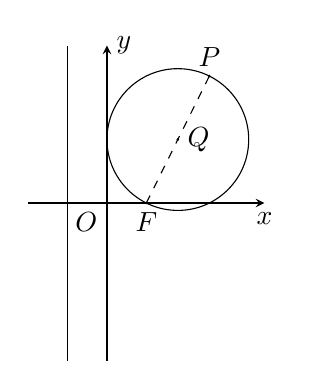
\begin{tikzpicture}
        \pgfmathsetmacro\xx{2}
        \pgfmathsetmacro\y{2}
        \pgfmathsetmacro\p{1}
        \pgfmathsetmacro\px{1.3}
        \pgfmathsetmacro\py{sqrt(2*(\px)))}
        \coordinate (O) at (0,0);
        \coordinate (F) at (\p/2,0);
        \coordinate (P) at (\px,\py);
        \coordinate (Q) at ($(P)!0.5!(F)$);
        \pgfmathsetmacro\r{sqrt((\px-\p/2)^2+\py^2)/2}
        \tkzInit[ymax=\y,ymin=-\y,xmax=\xx,xmin=-1] 
        \tkzFctPar[samples=400,domain=-2:2]{t**2/(2*\p)}{t}
        \draw[-stealth] (-1,0) -- (\xx,0) node [below] {$x$};
        \draw[-stealth] (0,-\y) -- (0,\y) node [right] {$y$};
        \fill (O) node [below left] {$O$} circle (0.5pt);
        \fill (F) node [below] {$F$} circle (0.5pt);
        \fill (P) node [above] {$P$} circle (0.5pt);
        \fill (Q) node [right] {$Q$} circle (0.5pt);
        \draw[dashed] (F) -- (P);
        \tkzVLine{-\p/2}
        \draw (Q) circle (\r);
    \end{tikzpicture}
\end{document}